\documentclass[12pt,a4paper]{article}

% Basic packages used for page layout, images, and spacing
\usepackage[a4paper,margin=1in]{geometry}
\usepackage{graphicx}
\usepackage{setspace}
\usepackage{parskip}

% Keep the document simple and readable
\setlength{\parindent}{0pt}
\onehalfspacing

\begin{document}

% ---------------------------------------------------------
% Assignment cover page
% ---------------------------------------------------------

\begin{center}

\vspace*{2cm}

{\Huge \textbf{HCI \& Computer Graphics}}

\vspace{0.5cm}

{\Huge \textbf{Assignment}}

\vspace{2.5cm}

{\Large \textbf{Partab Rai}}

\vspace{0.5cm}

{\Large \textbf{Computer Science}}

\vspace{0.4cm}

{\Large \textbf{Part III (P.E) Morning}}

\vspace{0.4cm}

{\Large \textbf{2k24/CSE/117}}

\end{center}

\newpage
% ---------------------------------------------------------
% Step 1 and HCI analysis
% ---------------------------------------------------------

\textbf{Step 1: Chosen App:}

Google Earth

\vspace{20pt}

\textbf{Step 2: Screenshots and Annotations:}

\textbf{Image 1 (HCI Focus):}

% The HCI screenshot is placed here
\begin{center}
    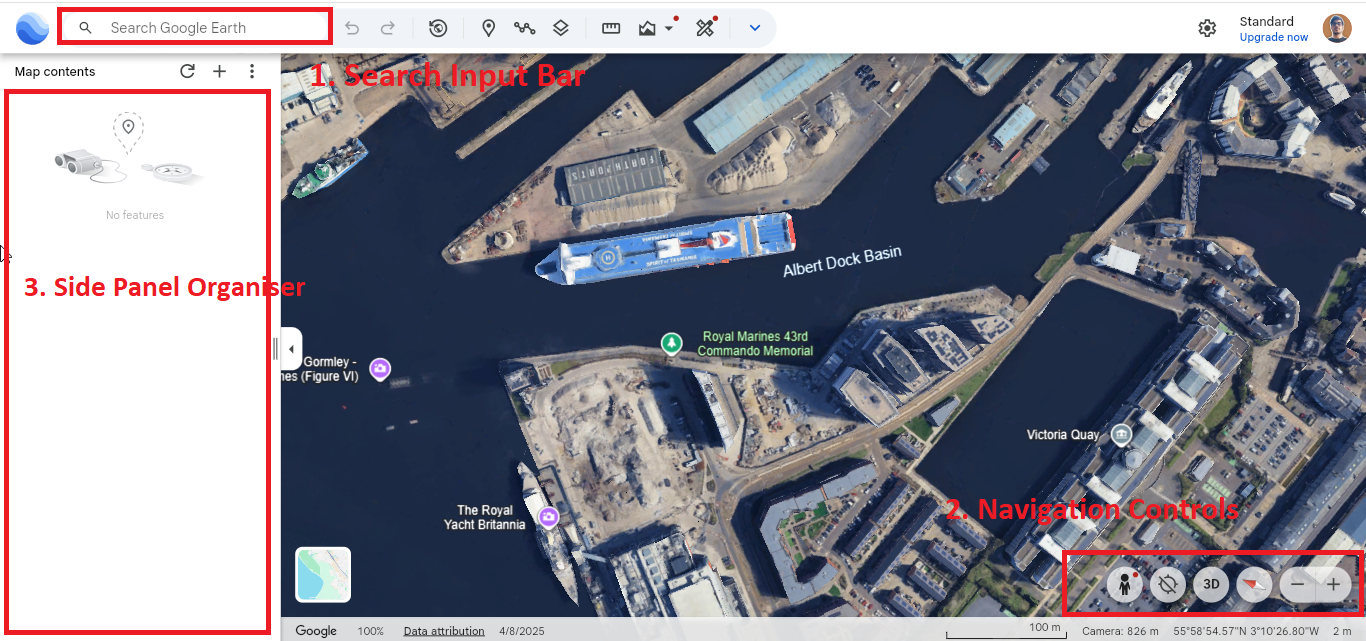
\includegraphics[width=\textwidth]{hci.png}
\end{center}

\vspace{20pt}

\textbf{1. Search Input Bar:}

It helps users quickly find a specific place, location, or area on Google Earth. Instead of manually moving around the map, the user can type a name or address and go directly to it. This saves time and makes finding locations much easier.

\vspace{20pt}

\textbf{2. Navigation Controls:}

They help users move around and explore the map. Users can zoom in or out, move the view, and change the direction they are looking from. This makes it easier to see a location closely or get a wider view of the surrounding area.

\vspace{20pt}

\textbf{3. Side Panel Organiser:}

It helps users keep their saved places and information organized. Users can view their saved locations, projects, and other map items from one place. This makes it easier to find and manage places they want to return to later.

\newpage

% ---------------------------------------------------------
% CG analysis
% ---------------------------------------------------------

\vspace{20pt}

\textbf{Image 2 (CG Focus):}

\vspace{10pt}

% The CG screenshot is placed here
\begin{center}
    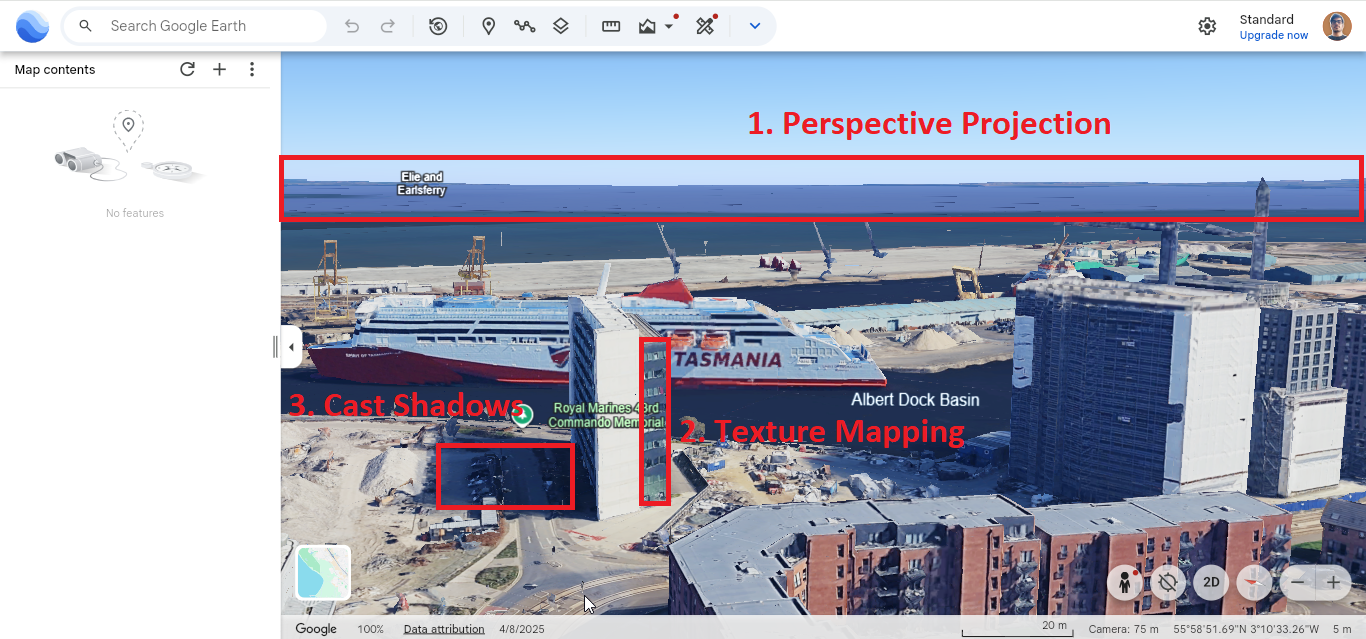
\includegraphics[width=\textwidth]{cg.png}
\end{center}

\vspace{20pt}

\textbf{1. Perspective Projection:}

It makes places look more realistic by showing objects the way they would appear from a real viewpoint. Objects that are closer look larger, while objects farther away look smaller. This helps users understand the shape, height, and distance of buildings, mountains, and other places.

\vspace{20pt}

\textbf{2. Texture Mapping:}

It adds real images and surface details to 3D objects and the ground. For example, buildings can show their actual walls, windows, and colors instead of looking like plain shapes. This makes locations look more realistic and easier to recognize.

\vspace{20pt}

\textbf{3. Cast Shadows:}

It shows shadows created by buildings, mountains, and other objects when light falls on them. This gives users a better idea of the height and shape of objects and makes the 3D view feel more like a real place.


\newpage

\textbf{Step 3: Reflection Questions:}

\vspace{20pt}

\textbf{1. How does the Computer Graphics quality help or hinder the user’s ability to interact with the software?}

Good graphics make the 3D environment easier to understand and explore. Clear buildings, terrain, textures, and shadows help users judge distance, height, size, and location more easily. Realistic visuals also make it easier to recognize roads, landmarks, and other places.

However, very high graphics quality can make the software slow, causing lag, longer loading times, and less smooth movement, especially on less powerful devices.


% ---------------------------------------------------------
% HCI improvement suggestion
% ---------------------------------------------------------

\vspace{20pt}


\textbf{2. What is one simple HCI change you would make to improve the user interface?}

I would add a visible button to quickly reset the camera to a top-down, north-facing view.
When users rotate or tilt the 3D view and become confused about their direction, they could return to a familiar view with one click. This would make navigation easier, especially for new users, without changing the existing controls.

\end{document}